\documentclass[conf]{new-aiaa}
%\documentclass[journal]{new-aiaa} for journal papers
\usepackage[utf8]{inputenc}

\usepackage{graphicx}
\usepackage{amsmath}
\usepackage[version=4]{mhchem}
\usepackage{siunitx}
\usepackage{longtable,tabularx}
\setlength\LTleft{0pt} 

\title{Proposal of Aerodynamic Innovations for an Aviary Optimization of a Short-Haul Single-Aisle Passenger Aircraft}

\author{Cooper T. Cook\footnote{Graduate Student, Department of Mechanical and Aerospace Engineering}}
\affil{University of California, Davis, California 95616}


\begin{document}

\maketitle

\section{Subsystem Definition \& Literature Synthesis}
\lettrine{M}{odern} aircraft design has seen significant aerodynamic innovation following improvements in simulation accuracy and ease of access. Following the beginning of aircraft design, specific technologies have been implemented into the conventional aircraft design process: wing sweep, supercritical wings, boundary layer laminarisation, wingtip devices, morphing airfoil geometry, and leading-edge anticontamination devices \cite{coelho_barbosa_aircraft_2023}. While implementation of more complex aerodynamic systems to improve aerodynamic efficiency is welcome in the sustainability effort, often the coupled performance of systems outside of aerodynamics is overlooked in the conventional design process, so the optimization of the aerodynamic subsystem does not lead to the optimization of the overall aircraft. This is why key improvements in overall aircraft efficiency are being made using multi-disciplinary design, analysis, and optimization (MDAO) \cite{leng_multidisciplinary_2025}. Focus on sustainability and emission reduction has led to innovations in aerodynamic efficiency, especially when coupled with the propulsion system in an MDAO framework \cite{bravo-mosquera_design_2022} or with many other subsystems \cite{press_of_acta_aero_et_astro_sinica_integrated_2026}. New aerodynamic configurations that more or less \emph{rely} on MDAO for the structural design process range from boxed-wing \cite{jemitola_analysis_2023} to blended wing body \cite{handa_recent_2022}.

In the effort to design a new short-range single-aisle passenger aircraft, my team, MicroRAPTORS, will implement an MDAO framework using Aviary \cite{gratz_aviary_2024}, an open-source framework for aircraft MDAO built on top of OpenMDAO \cite{gray_openmdao_2019}. My role in the team will be to develop the aerodynamic subsystem and its integration into Aviary. There are several subsystems that realistically couple with aerodynamics, which I will be integrating changes with. The primary subsystem I will be working with is the geometry/structure subsystem to ensure a physically feasible wing will be designed within the optimizer. We expect that a purely aerodynamic optimization of the aircraft will lead to impossible or highly impractical designs, so stress analysis, mass analysis, and cost analysis of the wing will need to be taken into account to find a practical design. The RFP for this short-range single-aisle passenger aircraft requests for a dramatic reduction in emissions, which---for the aerodynamic subsystem---means significantly improving aerodynamic efficiency alongside the propulsion system.

As mentioned previously, some recent advances in aerodynamic design have been in blended wing body aircraft \cite{handa_recent_2022} and morphing airfoil geometry \cite{coelho_barbosa_aircraft_2023}. These have previously been infeasible to implement in a traditional aircraft design process because of the complex coupling of the subsystems, shape and technology for manufacturing, and aerodynamic analysis. However, with advances in materials, computational power, simulation techniques, and MDAO, blended wing body aircraft and morphing airfoil geometry now appear more feasible \cite{majid_status_2021, handa_recent_2022}. One primary advantage of blended wing body aircraft over conventional aircraft is the reduced parasitic drag due to the lower wetted aircraft area. Additionally, a significant portion of the overall lift of the aircraft is created by the main body of the aircraft \cite{handa_recent_2022}. With morphing camber wings, the primary advantage is ability to optimize the wing shape mid-flight for reduced drag, increased lift, or increased maneuverability, without the addition of surface roughness typically attributed to conventional flaps and other control surfaces.

\section{Proposed Innovation \& Feasibility}
Blended wing body aircraft have been a popular area of study due to their aerodynamic efficiency advantages over conventional aircraft designs. This is why I propose to implement a blended wing body design as part of my subsystem in the Aviary framework. If time permits, I also aim to implement a morphing-camber design. 

Instead of conventional design's emperical equation-based aerodynamic analysis methods, I will implement automated analysis in Athena Vortex Lattice (AVL) and FlightStream using my automated mesh generation tool for morphing aircraft analysis. Using data from both of these analyses, I will consider training a multi-fidelity surrogate model for use within the Aviary optimizer to potentially reduce computational time. However, I expect that the number of iterations in the Aviary optimizer will not be enough to justify a surrogate model implementation. Development of this system is critical for MicroRAPTORS's success in meeting the emission reduction requirements of the RFP.

\begin{figure}[hbt!]
\centering
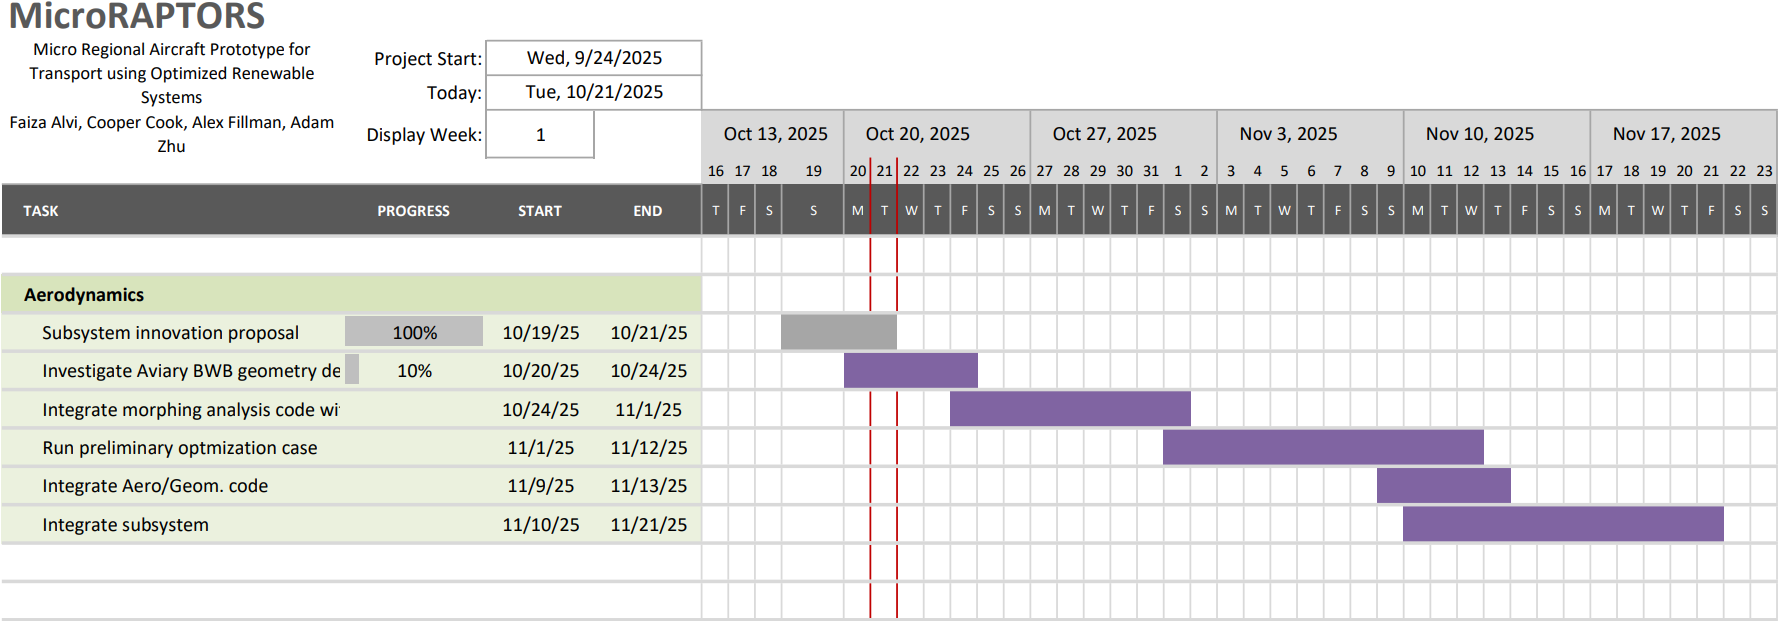
\includegraphics[width=1\textwidth]{cooper-gantt-chart.png}
\caption{Gantt chart timeline for aerodynamic subsystem creation and integration.}
\label{fig:cooper-gantt-chart}
\end{figure}

With the goal to create and implement the aerdynamic subsystem by the project's deadline, the timeline is relatively short and strict. So, the only thing that can change is the \emph{extent to which I will implement both blended wing body geometry and morphing camber}. I believe that blended wing body geometry alone is an appropriate goal for the timeline, considering I already have an analysis framework working. Adding a morphing camber feature will be a reach goal that I can consider once I have the initial aerodynamic subsystem working with the blended wing body.

The code for this project will be stored and updated on my GitHub repository at \url{
https://github.com/coopertomcook/mae298-cook}. The README will be kept current with up-to-date information about the state of the subsystem.

\bibliography{MAE_298}

\end{document}